\section{Непрерывный инструмент}

\begin{frame}{Инструменты в неэкспериментальных исследованиях}


  \begin{itemize}
      \item \href{https://www.aeaweb.org/articles?id=10.1257/aer.91.5.1369}{Acemoglu D., S. Johnson and J. A. Robinson. The Colonial Origins of Comparative Development: An Empirical Investigation, American Economic Review, 2001, vol. 91(5)}
      \item Авторы проверяют гипотезу, что качество институтов (индекс защиты прав собственности) имеет значение для обеспечения высоких темпов экономического роста, т.к. даёт преимущество в накоплении капитала.
      \item Выборка - страны Африки, Азии, Южной Америки, Океании
      \item Проблема - возможна двусторонняя связь.
  \end{itemize}
\end{frame}

\begin{frame}{Поиск инструмента}
  \begin{itemize}
      \item Инструмент не должен коррелировать с современными "шоками" (свойство экзогенности)
      \item Инструмент должен коррелировать с современным качеством институтов (свойство релевантности)
       
 \end{itemize}
\end{frame}

\begin{frame}{Поиск инструмента}
  \begin{itemize}
    \item Важна история колоний. Два типа колоний: <<extractive states>> типа Конго и s “Neo-Europes” типа Новой Зеландии
      \item Инструмент - смертность первых колонистов
      \item Логика: смертность колонистов => укоренение поселений европейцев => утверждение постоянных правил - "ранних институтов защиты прав собственности" до 1900 г. => современные институты защиты прав собственности в конце 20 века => накопление капитала => долгосрочный рост к 1995 г. 
 \end{itemize}
\end{frame}

\section{Инструменты Бартика}


\begin{frame}{Рост импорта из Китая и падение занятости в промышленном секторе США? \href {https://www.aeaweb.org/articles?id=10.1257/aer.103.6.2121}{(D.Autor, 2013)}}
% сюда нужен график
  \begin{figure}
   \centering
    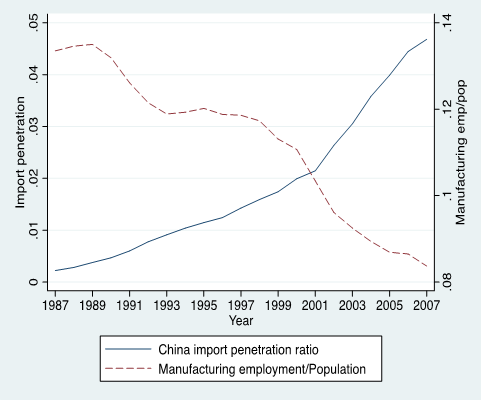
\includegraphics[width=\textwidth]{Lecture_Sources/Images/Bartik_import.png}
  \end{figure}
\end{frame}



\begin{frame}{Как оценить?}
%формулы
  \begin{itemize}
      \item$Y_{it}=\beta_0+\beta_1*X_{it}+\epsilon_{it}$ , где
      \item $Y_{it}$ -- изменение занятости в промышленном секторе в муниципалитете i в году t
      \item $X_{it}$ -- рост импорта промышленных товаров из Китая в муниципалитет i в году t
      \item $\epsilon_{it}$ -- <<случайные шоки>> в муниципалитете i в году t
      \item Проблема -- confounders, одновременно влияющие и на занятость, и на импорт
      \item Нужен инструмент
  \end{itemize}
\end{frame}

\begin{frame}{Импорт из Китая вырос по-разному в разных округах и штатах (CZ)}
 \begin{figure}
 \centering
       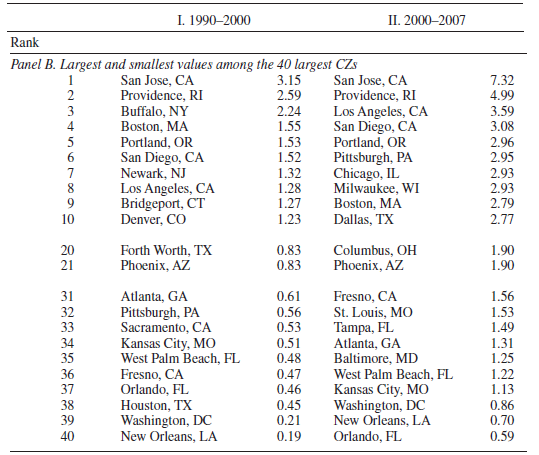
\includegraphics[width=\textwidth]{Lecture_Sources/Images/Bartik_differences.png}
  \end{figure}
\end{frame}

\begin{frame}{Разложение импорта по отраслям}
    \begin{itemize}
      \item$X_{it}=\sum\limits_{k=1}^K(S_{i,k,t}*g_{k,t}^{US})$ , где
      \item $X_{it}$ -- рост импорта всех промышленных товаров из Китая в округ i в году t
      \item $S_{i,k,t}$ -- доля отрасли k в округе i в году t
      \item $g_{k,t}^{US}$ --  рост импорта товаров отрасли k из Китая в США в году t
      \item k -- отрасль (электроприборы, одежда, обувь, игрушки, мебель...)
  \end{itemize}
\end{frame}

\begin{frame}{Общий тренд в росте импорта из Китая во все развитые страны}
%картинка- таблица с ростом импорта из Китая во все развитые страны
 \begin{figure}
 \centering
       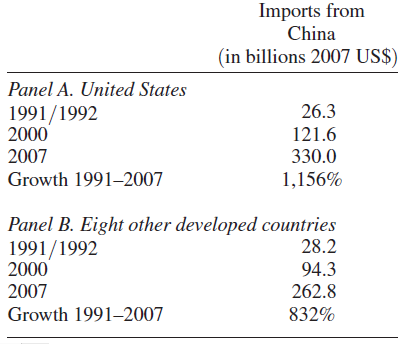
\includegraphics[width=250]{Lecture_Sources/Images/Bartik_common_trends.png}
  \end{figure}
 \end{frame}
 
\begin{frame}{Инструмент Бартика (shift-share IV)}
    \begin{itemize}
          \item$B_{it}=\sum\limits_{k=1}^K(S_{i,k,t-1}*g_{k,t}^{OHI})$ , где
      \item $S_{i,k,t}$ -- доля отрасли k в округе i в году t-1
      \item $g_{k,t}^{OHI}$ --  рост импорта товаров отрасли k из Китая в другие развитые страны в году t
      \item Инструмент коррелирует с $X_{it}$, но не коррелирует с местными шоками года t. 
    \end{itemize}
\end{frame}

\begin{frame}{Двухшаговая оценка}
%формулы
  \begin{itemize}
      \item Первый шаг
      \item $X_{it}=\gamma_0+\gamma_1*B_{it}+u_{it}$  
      \item Второй шаг
      \item $Y_{it}=\beta_0+\beta_1*\widehat{X_{it}}+\epsilon_{it}$
  \end{itemize}
\end{frame}

\begin{frame}{Рост импорта из Китая на каждую 1000\$ снижает занятость в пром.секторе на 0.6 п.п.}
%картинка- таблица с результатами 
   \begin{figure}
   \centering
       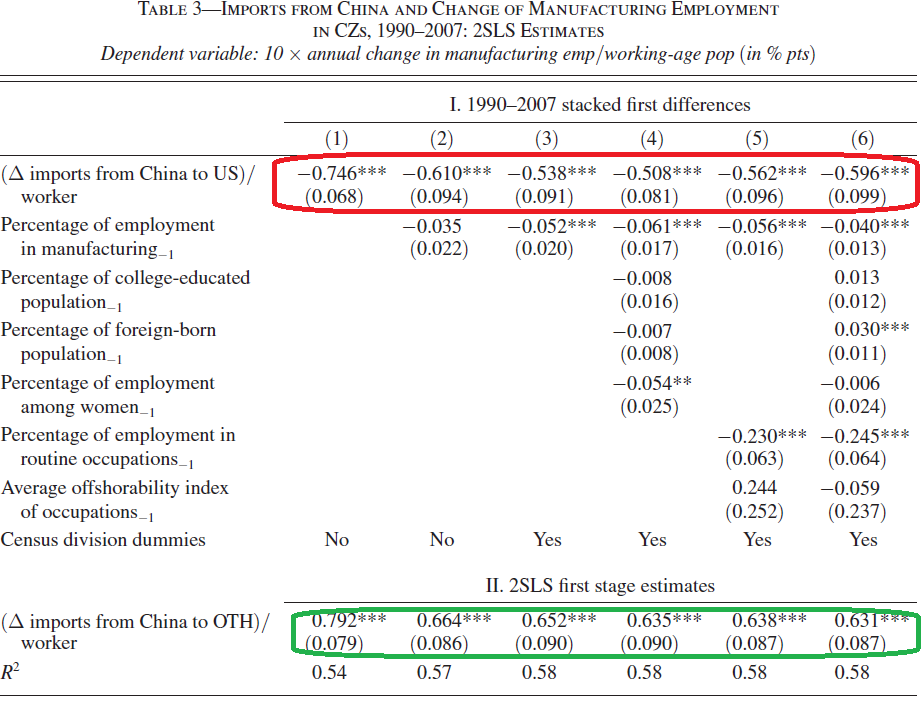
\includegraphics[width=\textwidth]{Lecture_Sources/Images/Bartik_results.png}
  \end{figure}
\end{frame}